\documentclass[tikz]{standalone}
\usepackage{fontspec}
\setmainfont{Latin Modern Roman}
\usetikzlibrary{positioning}

\definecolor{xcolor}{HTML}{3773b0}
\definecolor{ycolor}{HTML}{a40e3a}
\definecolor{zcolor}{HTML}{30a64d}

\begin{document}
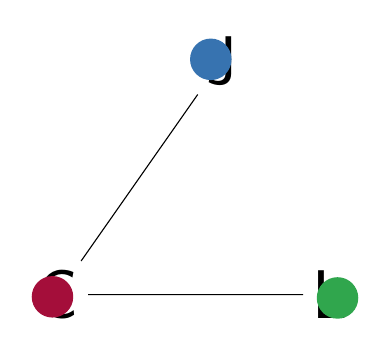
\begin{tikzpicture}[font=\sffamily]
  \node (j) at (80:2cm) {\fontsize{60}{72}\selectfont J};
  \node (x) at (83.86:2.0cm) {};
  \node (c) at (210:2cm) {\fontsize{60}{72}\selectfont C};
  \node (y) at (209.77:2.07cm) {};
  \node (l) at (-30:2cm) {\fontsize{60}{72}\selectfont L};
  \node (z) at (-29.75:2.1cm) {};
  \draw (j) -- (c) -- (l) -- cycle;
  \foreach \i in {x,y,z}
    \fill[\i color] (\i.center) circle[radius=7.5pt];
\end{tikzpicture}
\end{document}
